%%%%%%%%%%%%%%%%%%%%%%%%%%%%%%%%%%%%%%%%%
% Beamer Presentation
% LaTeX Template
% Version 1.0 (10/11/12)
%
% This template has been downloaded from:
% http://www.LaTeXTemplates.com
%
% License:
% CC BY-NC-SA 3.0 (http://creativecommons.org/licenses/by-nc-sa/3.0/)
%
%%%%%%%%%%%%%%%%%%%%%%%%%%%%%%%%%%%%%%%%%

%----------------------------------------------------------------------------------------
%	PACKAGES AND THEMES
%----------------------------------------------------------------------------------------

\documentclass{beamer}
% \documentclass[handout]{beamer}


\mode<presentation> {

\usetheme{Madrid}

}

\definecolor{DataBlue}{rgb}{0.50, 0.85, 0.99} 

\setbeamercolor{titlelike}{parent=structure,bg=black, fg = white}
\setbeamercolor{frametitle}{fg=white}
\usepackage{graphicx} % Allows including images
\usepackage{booktabs} % Allows the use of \toprule, \midrule and \bottomrule in tables
\usepackage[export]{adjustbox}
\usepackage[portuguese]{babel}
\usepackage[utf8]{inputenc}

\usepackage{pgfplots}
\usepackage{tikz}
\usetikzlibrary{calc,babel,quotes,angles}
\usepackage{tkz-euclide}

\usepackage{amsmath, amsfonts, amssymb}

\usepackage{cancel}

\usepackage{multirow}
% \usepackage{xcolor}

\makeatletter
\let\save@measuring@true\measuring@true
\def\measuring@true{%
  \save@measuring@true
  \def\beamer@sortzero##1{\beamer@ifnextcharospec{\beamer@sortzeroread{##1}}{}}%
  \def\beamer@sortzeroread##1<##2>{}%
  \def\beamer@finalnospec{}%
}
\makeatother


%----------------------------------------------------------------------------------------
%	TITLE PAGE
%----------------------------------------------------------------------------------------

\title{Geometria} %% Title
\subtitle{Aula 02}
\author{Gustavo Ale} % Your name
\institute[UFMT] % Your institution as it will appear on the bottom of every slide, may be shorthand to save space
{
EduCursinho - Faculdade de Engenharia \\ % Your institution for the title page
\medskip
\textit{gustavo.engca@gmail.com} % Your email address
}
\date{\today} % Date, can be changed to a custom date

% Rodapé
% \setbeamertemplate{footline}{%
%     \begin{beamercolorbox}[wd=\paperwidth]{footlinecolor}
%         \includegraphics[width=\paperwidth]{images/footbar.png}
%     \end{beamercolorbox}%
% }

\begin{document}
{
\setbeamertemplate{footline}{}
\begin{frame}
    \begin{columns}
        \begin{column}{0.48\textwidth}
            % \hspace*{-1cm}
            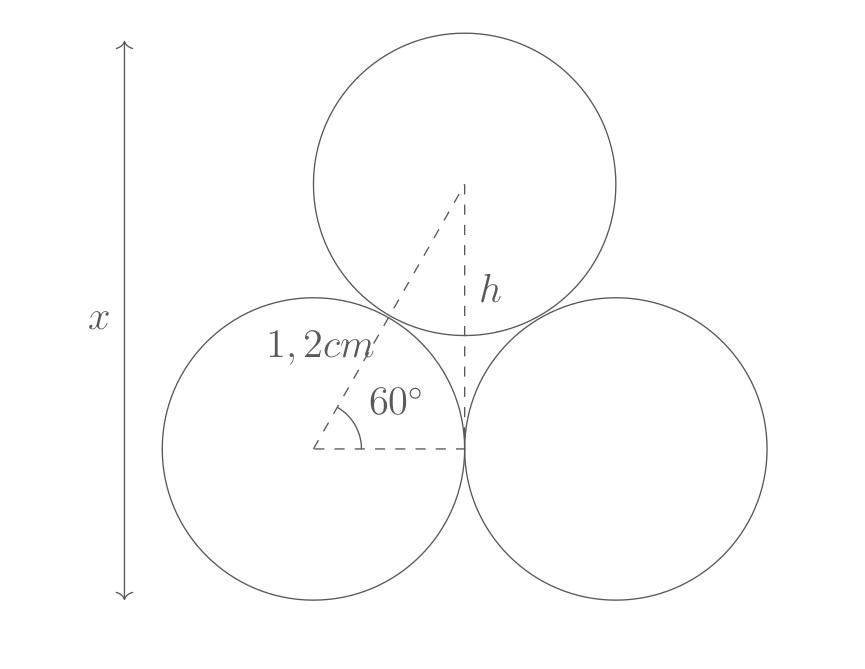
\includegraphics[width=\columnwidth,left]{../assets/geo.png}
        \end{column}
        \begin{column}{0.48\textwidth}
            \titlepage
        \end{column}
    \end{columns}

\end{frame}
}

%-------------------------------------------------------------------------------
% Sumário
%-------------------------------------------------------------------------------

\begin{frame}
    \frametitle{Sumário} % Table of contents slide, comment this block out to remove it
    \tableofcontents % Throughout your presentation, if you choose to use \section{} and \subsection{} commands, these will automatically be printed on this slide as an overview of your presentation
\end{frame}

%----------------------------------------------------------------------------------------
%	PRESENTATION SLIDES
%----------------------------------------------------------------------------------------

\section{Componentes das fíguras geométricas}
\subsection{Ponto, vértice}
\begin{frame}\frametitle{\subsecname}
    A primeira componente das fíguras geométricas e a mais simples delas é o ponto, o mesmo deve ser imaginado como um
    ponto infinitesimal, não possuindo comprimento, área ou perímetro. Quando um ponto é integrante de uma fígura
    geométrica o mais comum é chamarmos ele de \textit{vértice}
    \begin{figure}[H]
        \centering
        %\resizebox{\columnwidth}{!}
        \caption{Triângulo com o vértice $A$ em realce }
        % \label{fig:vertice_tri}
    \end{figure}

\end{frame}

\begin{frame}\frametitle{\subsecname}
    A partir de dois pontos $A$ e $B$ podemos traçar uma reta $\overline{AB}$ entre eles e caso exista um terceiro ponto $C$ sob a mesma reta,
    então esses três pontos são \textbf{colineares}.

    \begin{figure}[H]
        \centering
        %\resizebox{\columnwidth}{!}
        \caption{Pontos colineares $A$,$B$ e $C$}
        \label{fig:reta_ab}
    \end{figure}
\end{frame}

%------------------------------------------------

\subsection{Reta, aresta}
\begin{frame}\frametitle{\subsecname}
    A reta é um conjunto de pelo menos dois pontos, no caso dois pontos quaisquer $A$ e $B$ podem gerar a reta $\overline{AB}$, como na fígura \ref{fig:reta_ab}.
    Assim como o ponto é idealmente infinitesimal a reta idealmente não possui espessura. Quando uma reta é parte
    integrante de uma fígura geométrica sua denominação é \textit{aresta}.

    \begin{figure}[H]
        \centering
        %\resizebox{\columnwidth}{!}
        \caption{Retas $\overline{AB}$,$\overline{BC}$ e $\overline{AC}$ do triângulo $ABC$}
        \label{fig:tri_abc}
    \end{figure}
\end{frame}

%------------------------------------------------

\subsection{Plano e superfície}
\begin{frame}\frametitle{\subsecname}
    Quando se tem 3 ou mais pontos o resultado da conexão deles é tido como superfície, plano ou fígura geométrica, 
    Uma excessão a isso são os círculos e as elipses que não possuem vértices. 

    \begin{figure}[H]
        \centering
        %\resizebox{\columnwidth}{!}{%
        \begin{tikzpicture}
            \coordinate (A) at (0,0);
            \coordinate (B) at (4,1);
            \coordinate (C) at (5,4);
            \coordinate (D) at (2,3);
            \draw (A)-- node[below] {$\overline{AB}$} (B) ;
            \draw (B)--(C) ;
            \draw (C)-- node[above] {$\overline{CD}$} (D) ;
            \draw (D)--(A) ;
            \node[circle, fill, label={left:$A$}, inner sep=2pt] at (A) {};
            \node[circle, fill, label={right:$B$}, inner sep=2pt] at (B) {};
            \node[circle, fill, label={right:$C$}, inner sep=2pt] at (C) {};
            \node[circle, fill, label={left:$D$}, inner sep=2pt] at (D) {};
        \end{tikzpicture}
        %}
        \caption{Um quadrilátero $ABCD$ com as arestas $\overline{AB}$ e $\overline{CD}$ realçadas}
    \end{figure}

\end{frame}

%------------------------------------------------

\subsection{Sólidos}
\begin{frame}\frametitle{\subsecname}
    No contexto de fíguras geométricas tridimenssionais, ou chamados sólidos, os sólidos podem ser formados por 4 ou
    mais pontos ou através manipulação de fíguras geométricas bidimensionais num espaço tridimenssional.
    Todos objetos físicos que conhecemos podem ser abstraídos como formas geométricas, independente da complexidade.

    \begin{figure}[H]
        \centering
        %\resizebox{\columnwidth}{!}{%
        \begin{tikzpicture}
            \coordinate (A) at (0,0);
            \coordinate (B) at (2,4);
            \coordinate (C) at (4,1);
            \coordinate (D) at (2,2);
            \draw (A)--(B) ;
            \draw (B)--(C) ;
            \draw (C)--(A) ;
            \draw[dashed] (D)--(A) ;
            \draw[dashed] (D)--(B) ;
            \draw[dashed] (D)--(C) ;
            \node[circle, fill, label={left:$A$}, inner sep=2pt] at (A) {};
            \node[circle, fill, label={right:$B$}, inner sep=2pt] at (B) {};
            \node[circle, fill, label={right:$C$}, inner sep=2pt] at (C) {};
            \node[circle, fill, label={left:$D$}, inner sep=2pt] at (D) {};
        \end{tikzpicture}
        %}
        \caption{Tetraedro, o objeto tridimenssional com menos faces}
    \end{figure}
\end{frame}

\begin{frame}\frametitle{\subsecname}
    %\columnbreak
    Grandezas notórias das componentes citadas:
    \begin{itemize}
        \setlength\itemsep{1.15pt}
        \item Ponto, vértice: distância relativo a outro objeto.
        \item Reta: comprimento, distância e ângulo relativos a outro objeto.
        \item Superfície: área, perímetro.
        \item Sólido: volume.
    \end{itemize}
\end{frame}
%------------------------------------------------

% \section{Notação científica}
% \begin{frame}\frametitle{\subsecname}
%     \begin{columns}
%         \column{0.45\textwidth}
%         \begin{figure}[H]
%             \centering
%             %\resizebox{\columnwidth}{!}{%
%             \begin{tikzpicture}
%                 \coordinate (A) at (2,2);
%                 \coordinate (B) at (4,2);
%                 \coordinate (C) at (2,0);
%                 \coordinate (D) at (2,4);
%                 \draw[cyan] (A)--node[below] {$r$}(B) ;
%                 \draw[orange] (C)--node[left] {$d$}(D) ;
%                 \draw[magenta] (A) circle (2cm)
%                 (0,3) node[left] {$c$};
%             \end{tikzpicture}
%             %}
%             \caption{Raio $r$, diâmetro $d$ e circunferência $c$ de um círculo}
%         \end{figure}

%         A circunferência do círculo é $2\pi r$.

%         \column{0.5\textwidth}
%         \begin{block}{Perímetro}
%             comprimento do contorno de uma fígura geométrica. \\
%         \end{block}

%         \begin{block}{Raio}
%             distância entre o centro de uma circunferência até seu contorno ou superfície.
%         \end{block}

%         \begin{block}{Diâmetro}
%             comprimento de reta que passe pelo centro da circunferência e cujo seus pontos de início e fim estejam sobre a circunferência
%         \end{block}

%         % \begin{block}{Circunferência}
%         %     perímetro de uma circunferência.
%         % \end{block}

%     \end{columns}

% \end{frame}

% %------------------------------------------------

% \subsection{Área}
% \begin{frame}\frametitle{\subsecname}
%     Área é a medida que expressa a quantidade de espaço bidimenssional ocupado por uma fígura geométrica. A unidade base
%     para área é o \textbf{metro quadrado (símbolo ${m^2}$)}. Seus múltiplos também acompanham o termo 'quadrado',
%     e a equivalência é a mesma do metro, porém elevada ao quadrado.
%     \pause Ex.:

%     \begin{align*}
%         1m   & = 100cm     \\
%         \pause
%         1m^2 & = (100cm)^2 \\
%         \pause
%         1m^2 & = 100^2cm^2
%     \end{align*}

% \end{frame}

% %------------------------------------------------

% \begin{frame}\frametitle{\subsecname}

%     \begin{figure}[H]
%         \centering
%         %\resizebox{\columnwidth}{!}{%
%         \begin{tikzpicture}
%             \coordinate (A) at (0,0);
%             \coordinate (B) at (4,3);
%             \coordinate (C) at (4,0);
%             % \coordinate (D) at (0,3);
%             \node[circle, fill, label={left:$A$}, inner sep=2pt] at (A) {};
%             \node[circle, fill, label={right:$B$}, inner sep=2pt] at (B) {};
%             \node[circle, fill, label={right:$C$}, inner sep=2pt] at (C) {};
%             % \node[circle, fill, label={left:$D$}, inner sep=2pt] at (D) {};
%             % \draw[dashed] (A)--(D)--(B);
%             \draw[fill=gray!25] (A)--(B)--(C)--(A);
%         \end{tikzpicture}
%         %}
%         \caption{Área é o espaço bidimenssional ocupado pela região cinza.}
%         \label{fig:tri_abc}
%     \end{figure}
% \end{frame}

% %------------------------------------------------

% \begin{frame}\frametitle{\subsecname}

%     \begin{table}[H]
%         \resizebox{0.5\columnwidth}{!}{%
%             \begin{tabular}{l|l|l}
%                 \textbf{Nome}       & \textbf{Sigla} & \textbf{Equivalência}       \\ \hline
%                 picometro quadrado  & $pm^2$         & $10^{-24}m^2$               \\
%                 nanometro quadrado  & $nm^2$         & $10^{-18}m^2$               \\
%                 micrometro quadrado & $\mu m$        & $10^{-12}m^2$               \\
%                 milimetro quadrado  & $mm^2$         & $10^{-6}m^2$                \\
%                 centímetro quadrado & $cm^2$         & $10^{-4}m^2$                \\
%                 decímetro quadrado  & $dm^2$         & $10^{-2}m^2$                \\
%                 metro quadrado      & $m^2$          & $1m^2$                      \\
%                 decâmetro quadrado  & $dam^2$        &                             \\
%                 are                 & $are$          & \multirow{-2}{*}{$100m^2$}  \\
%                 hêctometro quadrado & $hm^2$         &                             \\
%                 hectare             & $ha$           & \multirow{-2}{*}{$10^4m^2$} \\
%                 quilometro quadrado & $km^2$         & $10^6m^2$
%             \end{tabular}%
%         }
%         %\caption{Unidades medida de área}
%     \end{table}
% \end{frame}

% %------------------------------------------------

% \subsection{Volume}

% \begin{frame}\frametitle{\subsecname}
%     O volume expressa
%     a quantidade de espaço tridimenssional ocupado por um objeto. No caso do volume existe duas unidades de medida base,
%     o \textbf{metro cúbico (símbolo $m^3$)} e o \textbf{litro}, ambos são usados regularmente, na qual o litro é a unidade mais usada para volumes
%     pequenos, enquanto o metro cúbico é usado para expressar volumes maiores.

%     \begin{align*}
%         1m   & = 100cm     \\
%         \pause
%         1m^3 & = (100cm)^3 \\
%         \pause
%         1m^3 & = 100^3cm^3
%     \end{align*}
% \end{frame}

% %------------------------------------------------

% \begin{frame}\frametitle{\subsecname}
%     \begin{figure}[H]
%         \centering
%         %\resizebox{0.5\columnwidth}{!}{%
%         \begin{tikzpicture}
%             \coordinate (A) at (0,0);
%             \coordinate (B) at (0,3);
%             \coordinate (C) at (3,3);
%             \coordinate (D) at (3,0);
%             \coordinate (E) at (1,1);
%             \coordinate (F) at (1,4);
%             \coordinate (G) at (4,4);
%             \coordinate (H) at (4,1);
%             \draw[fill=gray!25] (A)--(B)--(F)--(G)--node[right]{$L$}(H)--node[right]{$L$}(D)--node[below]{$L$}(A);
%             \draw (B)--(C)--(D);
%             \draw (C)--(G);
%             \draw[dashed] (A)--(E)--(H);
%             \draw[dashed] (E)--(F);
%         \end{tikzpicture}
%         %}
%         \caption{Cubo, cujo volume se dá por $L^3$, onde $L$ é o comprimento das arestas}
%     \end{figure}
% \end{frame}

% %------------------------------------------------

% \begin{frame}\frametitle{\subsecname}
%     \begin{table}[H]
%         \resizebox{0.5\columnwidth}{!}{%
%             \begin{tabular}{l|l|l}
%                 \textbf{Nome}     & \textbf{Sigla} & \textbf{Equivalência}          \\ \hline
%                 milimetro cúbico  & $mm^3$         & $10^{-9}m^3$                   \\ \hline
%                 centímetro cúbico & $cm^3$         &                                \\
%                 mililitro         & $ml$           & \multirow{-2}{*}{$10^{-6}m^3$} \\ \hline
%                 decímetro cúbico  & $dm^3$         &                                \\
%                 litro             & $l$            & \multirow{-2}{*}{$10^{-3}m^3$} \\ \hline
%                 metro cúbico      & $m^3$          & $1m^2$                         \\ %\hline                      
%             \end{tabular}%
%         }
%         %\caption{Unidades medida de volume}
%     \end{table}
% \end{frame}

% %------------------------------------------------
% \subsection{Ângulo}

% \begin{frame}\frametitle{\subsecname}
%     Ângulo é uma medida de inclinação entre duas retas ou dois planos, desde que eles não sejam paralelos entre si, no
%     contexto da geometria os ângulos estão presentes em todos os vértices das fíguras geométricas.
%     As unidades de medida mais comuns para ângulo são \textbf{graus} (símbolo $^{\circ}$), \textbf{radianos} (símbolo $rad$) e \textbf{gradianos} (símbolo $gon$).

%     Quanto no escopo das funções trigonométricas a unidade de medida mais utilizada é o radiano, por outro lado,
%     em aplicações de engenharia e na geometria a unidade mais usada é o grau. Considerando um grau $\alpha$ em graus,
%     sua conversão para radianos se dá por $rad(\alpha) = \alpha\cdot\pi/180$

% \end{frame}

% %------------------------------------------------

% \begin{frame}[fragile]\frametitle{\subsecname}
%     \begin{figure}[H]
%         \centering
%         %\resizebox{\columnwidth}{!}{%
%         \begin{tikzpicture}
%             \coordinate (O) at (1,2);
%             \coordinate (A) at (0.5,1);
%             \coordinate (B) at (2.5,5);
%             \coordinate (C) at (0,2);
%             \coordinate (D) at (5,2);
%             \draw (A)--(B) node[above] {$p$};
%             \draw (C)--(D) node[above] {$q$};
%             % \draw (O) node[above right] {$65^\circ$};
%             % \pic[angle radius=1cm,"$\alpha$"] {angle=a--b--c};
%             \pic ["$65^\circ$", draw, -, angle eccentricity=2] {angle = D--O--B};
%             % \draw (B)--(C);
%             % \draw (A)--(C);
%         \end{tikzpicture}
%         %}
%         \caption{Ângulo entre as retas $p$ e $q$}
%     \end{figure}
% \end{frame}

% %------------------------------------------------

% \begin{frame}[fragile]\frametitle{\subsecname}
%     Uma reta $p$ é \textbf{perpendicular} a reta $q$ se o ângulo formado entre elas for de 90 graus.
%     \begin{figure}[H]
%         \centering
%         %\resizebox{\columnwidth}{!}{%
%         \begin{tikzpicture}
%             \coordinate (O) at (1,1.5);
%             \coordinate (A) at (0,2);
%             \coordinate (B) at (4,0);
%             \coordinate (C) at (0,0);
%             \coordinate (D) at (3,4.5);
%             \draw (A)--(B) node[above] {$p$}  ;
%             \draw (C)--(D) node[left] {$q$};
%             % \pic[angle radius=1cm,"$\alpha$"] {angle=a--b--c};
%             \pic ["$90^{\circ}$", draw, -, angle eccentricity=2] {angle = B--O--D};
%             % \draw (B)--(C);
%             % \draw (A)--(C);
%         \end{tikzpicture}
%         %}
%         \caption{Retas perpendiculares $p$ e $q$}
%     \end{figure}
% \end{frame}

% %------------------------------------------------

% \begin{frame}[fragile]\frametitle{\subsecname}
%     Duas retas $p$ e $q$ são consideradas \textbf{paralelas entre si}, se qualquer reta $r$ perpendicular a reta $p$ também for
%     perpendicular a reta $q$. Outra forma de descrever retas paralelas é através do \textbf{Quinto Postulado de Euclides}
%     que diz: Supondo que duas retas $p$ e $q$ são cortadas por uma terceira reta $r$. Se a soma dos ângulos formados um
%     mesmo lado da reta $r$ resultar em 180 graus, então $m$ e $n$ são retas paralelas entre si.

%     \begin{figure}[H]
%         \centering
%         %\resizebox{\columnwidth}{!}{%
%         \begin{tikzpicture}
%             \coordinate (A) at (0,0);
%             \coordinate (B) at (5,1);
%             \coordinate (C) at (0,2);
%             \coordinate (D) at (5,3);
%             \draw (A)--node[below] {$p$}(B) ;
%             \draw (C)--node[above] {$q$}(D) ;
%         \end{tikzpicture}
%         %}
%         \caption{Retas paralelas $p$ e $q$}
%     \end{figure}
% \end{frame}

%------------------------------------------------

\subsection{Exercícios da última aula}
\begin{frame}\frametitle{\subsecname}
    \begin{block}{Exercícios}
        Converta:
        \begin{itemize}
            \item a) $1903m$ para $mm$
            \item b) $17km$ para $m$
            \item c) $10cm^3$ para $dm^3$
            \item d) $20L$ para $m^3$
            \item e) $2ha$ para $m^2$
            \item f) $2\pi$ para graus
        \end{itemize}
    \end{block}
\end{frame}

%------------------------------------------------

\begin{frame}\frametitle{\subsecname}
    a)
    \begin{align*}
        1903m &\rightarrow ? mm\\ \pause
        1m &= 1000mm \\ \pause
        1903\cdot1m&=1903000mm\\
    \end{align*}
\end{frame}

\begin{frame}\frametitle{\subsecname}
    b)
    \begin{align*}
        17km &\rightarrow ? m\\ \pause
        1km &= 1000m \\ \pause
        17\cdot1m&=17000m\\
    \end{align*}
\end{frame}

\begin{frame}\frametitle{\subsecname}
    c)
    \begin{align*}
        10cm^3 &\rightarrow ? dm^3\\ \pause
        1cm^3 &= 10^{-6}m^3 \\ \pause
        1dm^3 &= 10^{-3}m^3 \\ \pause
        \therefore 1cm^3&=10^{-3}dm^3\\ \pause
        10cm^3 &= 10^{-2}dm^3
    \end{align*}
\end{frame}

\begin{frame}\frametitle{\subsecname}
    d)
    \begin{align*}
        20L &\rightarrow ? m^3\\ \pause
        1L &= 10^{-3}m^3 \\ \pause
        20\cdot 1L&=20\cdot10^{-3}m^3\\ \pause
        20L &= 2\cdot 10^{-2}m^3
    \end{align*}
\end{frame}

\begin{frame}\frametitle{\subsecname}
    e)
    \begin{align*}
        2ha &\rightarrow ? m^2\\ \pause
        1ha &= 10^{4}m^2 \\ \pause
        2\cdot 1ha&=2\cdot10^{4}m^2
    \end{align*}
\end{frame}

\begin{frame}\frametitle{\subsecname}
    f)
    \begin{align*}
        2\pi \text{(rad)} &\rightarrow ? \text{(graus)}\\[1ex] \pause
        \text{(graus)} &= \frac{180}{\pi}\cdot\text{(rad)} \\[1ex] \pause
        \text{(graus)} &= \frac{180}{\pi}\cdot2\pi \\[1ex] \pause
        \text{(graus)} &= \frac{180}{\cancel{\pi}}\cdot2\cancel{\pi} \\[1ex]\pause
         &= 360^\circ
    \end{align*}
\end{frame}

%------------------------------------------------

\begin{frame}
    \Huge{\centerline{Perguntas?}}
\end{frame}

%----------------------------------------------------------------------------------------

\end{document}